\documentclass[journal]{./IEEE/IEEEtran}
\usepackage{cite,graphicx,textcomp}

\newcommand{\SPTITLE}{Off-Campus Housing Service}
\newcommand{\ADVISEE}{Marian M. Alvarez}
\newcommand{\ADVISER}{Katrina Joy Magno}

\newcommand{\BSCS}{Bachelor of Science in Computer Science}
\newcommand{\ICS}{Institute of Computer Science}
\newcommand{\UPLB}{University of the Philippines Los Ba\~{n}os}
\newcommand{\REMARK}{\thanks{Presented to the Faculty of the \ICS, \UPLB\
                             in partial fulfillment of the requirements
                             for the Degree of \BSCS}}
        
\markboth{CMSC 190 Special Problem, \ICS}{}
\title{\SPTITLE}
\author{\ADVISEE~and~\ADVISER%
\REMARK
}
\pubid{\copyright~2014~ICS \UPLB}


%%%%%%%%%%%%%%%%%%%%%%%%%%%%%%%%%%%%%%%%%%%%%%%%%%%%%%%%%%%%%%%%%%%%%%%%%%

\begin{document}

% TITLE
\maketitle


% INTRODUCTION
\section{Introduction}

\subsection{Background of the Study}
Based on the data in Table 1, an average of 9000 students coming from different regions in the Philippines were enrolled in the university during second semester AY 2013-2014 with OSAM profiles. Students, especially those from far-away places, need a housing facility within the vicinity of the campus. However, the university residence halls can only accommodate 2,446 students, based on the data in Table 2, and most of the dormitories handled by the university can only accommodate freshmen students. They will end up looking for decent dormitories and apartments outside the campus. This will be hard for them since they are not yet familiar with the area. The upperclassmen, on the other hand, are also having a hard time finding a new place to stay because of their busy schedule. Due to this reasons, a facility that will allow students to search for an off-campus housing will be of help. Since Internet is already available inside and outside the campus, a web application for this type of service will provide an efficient way of finding an off-campus housing for students. They can choose a dormitory or an apartment based on their liking with the help of other students that would give reviews about the particular place. They can check the photos of the dormitories and apartments that are uploaded by the users. This can also be used by the property owners to advertise their dormitory or apartment.
\subsection{Statement of the Problem}
One of Chancellor Rex Victor O. Cruz's Five (5) Point Thematic Action Agenda is to develop a system for assisting students find decent and affordable accommodation \cite{electronic_mv}.  This includes ensuring the quality and safety of the students in and off campus. At this time, however, only UHO, which provides in-campus housing service, can directly reach the students and owners of off-campus housing services just advertise through flyers and posters.
Finding an appropriate place to stay in is  a necessity for freshmen students who are not given a slot in any university residence halls. Going to Los Ban\~{n}os before the start of the semester just to find a place to stay near the university will be costly especially to those who live in faraway places. This has been a problem for upperclassmen students as well, since most of them are busy with their academics and other extra curricular activities and they do not have an ample time to search for a possible place to stay.
\begin{table}
	\centering
	\caption{Number of Students Enrolled in University of the Philippines per Region \cite{misc_t}} 
    \begin{tabular}{ | p{1.5cm} | p{1.5cm} |}
    \hline
   	Region & Number of Students \\ \hline
    ARMM & 3 \\ \hline
    CAR & 46 \\ \hline
    NCR & 1439 \\ \hline
    I & 73 \\ \hline
    II & 157 \\ \hline
    III & 812 \\ \hline
    IV-A & 4767 \\ \hline
    IV-B & 264 \\ \hline
    IX & 76 \\ \hline
    V & 283 \\ \hline
    VI & 20 \\ \hline
    VII & 17 \\ \hline
    VIII & 292 \\ \hline
    X & 38 \\ \hline
    XI & 23 \\ \hline
    XII & 20 \\ \hline
    XIII & 71 \\ \hline
    Unspecified & 578 \\ \hline
    TOTAL & 8979 \\ \hline
    \end{tabular}
    
	\end{table}	

If the university can provide a web-application for Off Campus Housing for the students, it would be easier for them to locate possible places for accommodation.
\subsection{Significance of the Study}
\begin{table}
	\centering
	\caption{University of Philippines- Los Ba\~{n}os Residence Halls Information }
    \begin{tabular}{ | p{1.5cm} | p{1.5cm} | p{1.5cm} | p{1.5cm}|}
    \hline
    Dormitory & Type &  Student Accommodating & Maximum Students \\ \hline
    Men's Residence Hall & Female & Freshmen & 646 \cite{electronic_men} \\ \hline
  	Women's Residence Hall & Female & Freshmen and Upperclassmen & 444 \cite{electronic_wmen} \\ \hline
  	New Dormitory & Co-Ed & Freshmen & 300 \cite{electronic_new} \\ \hline
  	Veterinary Medicine Residence Hall & Co-Ed & Freshmen and Upperclassmen & 280 \cite{electronic_vet} \\ \hline
  	New Forestry Residence Hall & Co-Ed & Freshmen and Upperclassmen & 156 \cite{electronic_nfrh} \\ \hline
  	Makiling Residence Hall & Male & Freshmen and Upperclassmen & 112 \cite{electronic_mareha} \\ \hline
  	Forestry Residence Hall & Female & Freshmen and Upperclassmen & 144  \cite{electronic_foreha} \\ \hline
  	Acci Dorm-Upper & Female & Freshmen & 56  \cite{electronic_au}\\ \hline
  	Acci Dorm-Lower & Male & Freshmen and Upperclassmen & 54  \cite{electronic_al} \\ \hline
  	ATI-NTC Residence Hall & Co-Ed & Freshmen & 130 \cite{electronic_ati} \\ \hline
  	International House & Co-Ed & International Graduate Students & 124 \cite{electronic_ih} \\ \hline
  	Total &&& 2446\\ \hline 
    \end{tabular}
    
	\end{table}	
Internet has been used by people nowadays in searching for different things, even a place to stay in.There are already websites that cater search engine for dormitories and apartments, however the locations are mainly in cities.  And it is hard searching online about dormitories and apartments around Los Ba\~{n}os.

By just using the Internet, students can search for dormitories and/or apartments and read reviews written by their schoolmates. 
\subsection{Objectives}
The general objective is to develop web application that can be used by students  to look for dormitories and apartments online.
\pubidadjcol
	\begin{itemize}
	\item To use OSAM System API for logging in to the web application.
    \item To use Google Maps API for tagging and locating dormitories and apartments
	\item To have a repository of information about dormitories and apartments around Los Ba\~{n}os.
	\item To implement a search engine for off-campus dormitories and apartments around Los Ba\~{n}os.
	\end{itemize}

\subsection{Scope and Limitations}
The Off-Campus Housing system will only focus on housing facilities around the Los Banos. Students can access this system if they have an OSAM account. 


% REVIEW OF RELATED LITERATURE
\section{Review of Related Literature}
\subsection{Web Search Engine}
Web Search Engine is a system developed for searching information on the internet. There are two major functions of search engines-crawling and building and index and providing results by calculating relevancy and serving results \cite{electronic_se}.  Many universities nowadays provides off-campus rental housing search engine to help their students find a place to stay. These search engines mostly use crowdsourcing. 
	\subsection{Features of other existing Off-Campus Housing Websites}
	\begin{enumerate}
		\item online searchable database / search listing
		\item roommate finder
		\item google maps integration
		\item accounts for students, parents, and property managers
		\item email the property managers directly
		\item downloadable lease contract
		\item photo gallery
		\item message boards
	\end{enumerate}
	\subsection{Variables used for searching:}

		\begin{enumerate}
		\item classification (dormitory, house, apartment, studio type, room for rent, mobile home, etc)
		\item rent fee
		\item expected move-in date
		\item maximum head count
		\item amenities (furnished, semi-furnished, has swimming pool, has rooftop, etc)
		\item pets allowed
		\item handicap accessibility
		\item activities allowed (smoking, drinking, group meetings, etc)
		\item lease length
		\item kilometers away from the university
		\item number of beds provided
		\item number of comfort rooms
		\end{enumerate}
\subsection{University in the Philppines that have an Off-Campus Housing Service}
Ateneo De Manila University \\
	-The Ateneo De Manila University provides a pdf file that includes a directory of Accredited Off-Campus Housing around Katipunan. Name of the dormitory, contact person, address, contact numbers, email address, classification, star rating, dormitory information, price range, and other amenities are included in the file. It also shows photos of the dormitories and a map. \cite{electronic_admu} \\
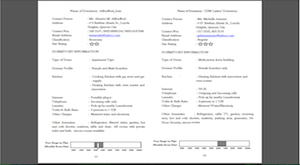
\includegraphics[scale=0.70]{images/admu2.png}	\\
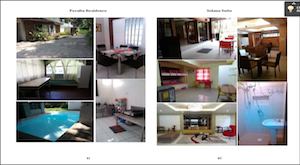
\includegraphics[scale=0.70]{images/admu3.png}
\subsection{Crowdsourcing}
Crowdsourcing is the process of obtaining information by getting contribution from a large group of people online. Famous example of croudsourcing is Wikipedia. One of the benefits of crowdsourcing is the ability of collecting large number of information at inexpensive cost. Additionally, it tends to get better quality of information since several people like to give their best ideas \cite{electronic_cs}. 
Four types of Crowdsourcing:
\begin{enumerate}
	\item Crowd Creation \\
		- Best known form of crowdsourcing. Creating a new writing, photography, music, film, or a software and make it available online.
	\item Crowd Wisdom \\
		- This attempts to use other people's knowledge in solving problems and predicting strategies in corporate world. Example of Crowd Wisdom are idea jams and prediction markets such as Iowa Elections Market. Hollywood Stock Exchange, and SIM Exchange. \cite{electronic_cst} 
	\item Crowd Voting \\
		- Used to get the people's judgment to organize and filter articles, music, movies, picture, and many more \cite{electronic_csw}. 
	\item Crowd Funding \\
		- It is the practice of funding a project or venture by raising many small amounts of money \cite{book_oxford}.
\end{enumerate}
\section{Methodology}
\subsection{Development Tools}
	The system will be developed under Ubuntu Operating System. To be able to implement the system, it will be necessary to install and use the following:
	 \begin{enumerate}
		\item Interface: Foundation will be used for the system's interface. Foundation is the most advanced front-end framework in the world \cite{electronic_foun} . It contains HTML and CSS-based design templates for typography, forms, buttons, navigation and other interface components, as well as optional JavaScript extensions.
		\item Framework: CodeIgniter 2.2.0 will be used for the implementation. It uses model-view-controller pattern in organization of files in programming.
		\item Programming Language: PHP5 is a scripting language that is suited for web developing. 
		\item Database: MySQL 5.1.41 will be used as database for this application. It is an open-source database management system.
	\end {enumerate} 
	\subsection{System Requirements Definition}
	This involved communicating with OSA to determine the system's requirements and functionalities. \\
	Functional Requirements \\
	
	-The system is to be used by three (3) types of users; these are the administrator, student, and the property manager. Each type of user is given different access privileges for the system:
		\begin{enumerate}
		\begin{figure} 
			\centering
			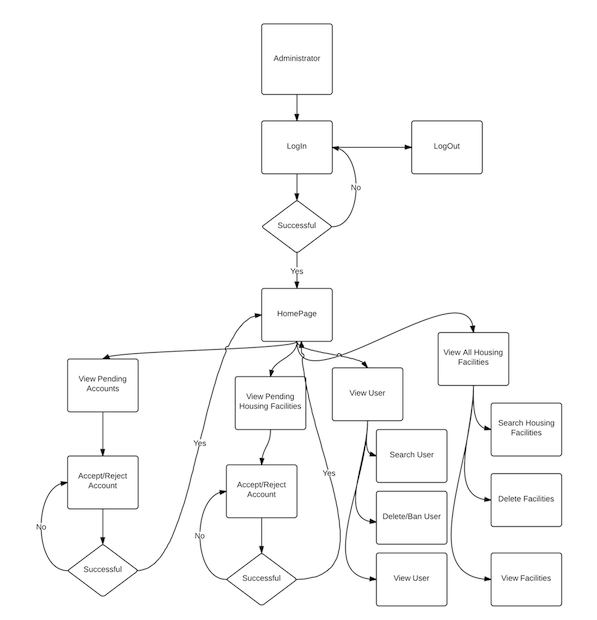
\includegraphics[width=10cm,height=12cm]{images/admin.png}
			\caption{Administrator Workflow Diagram}
		
		\end{figure}
		\item The administrator is capable of performing the following system functions:
		
			\begin{itemize}
				\item Approve, delete, and view properties added by the students and property managers.
				\item Search dormitories and apartments by :
					\begin{itemize}
						\item curfew
						\item users of the comfort rooms (shared / exclusive)
						\item bathing type (shower / pail)
						\item toilet facility (pail system, flush toilet, pit toilet) 
						\item deposit/advanced rent required
						\item rent payment (bank, cash, post-dated checks)
						\item sex (male only / female only / coed)
						\item distance of nearest sari-sari store in meters
						\item security features (has 24/7 guard, has night guard, has CCTV, landlord/landlady lives nearby, relies on good luck)
						\item electric/water billing (paid to landlord/landlady, paid to meralco/laguna water)
						\item internet availability (free wifi, paid wifi, bring your own, not allowed)
						\item transportation to university and approximate transportation time

					\end{itemize}
				\item Approve, delete, and view property managers.
				\item Add, edit and delete announcements.
			\end{itemize}
			\begin{figure} 
			\centering
			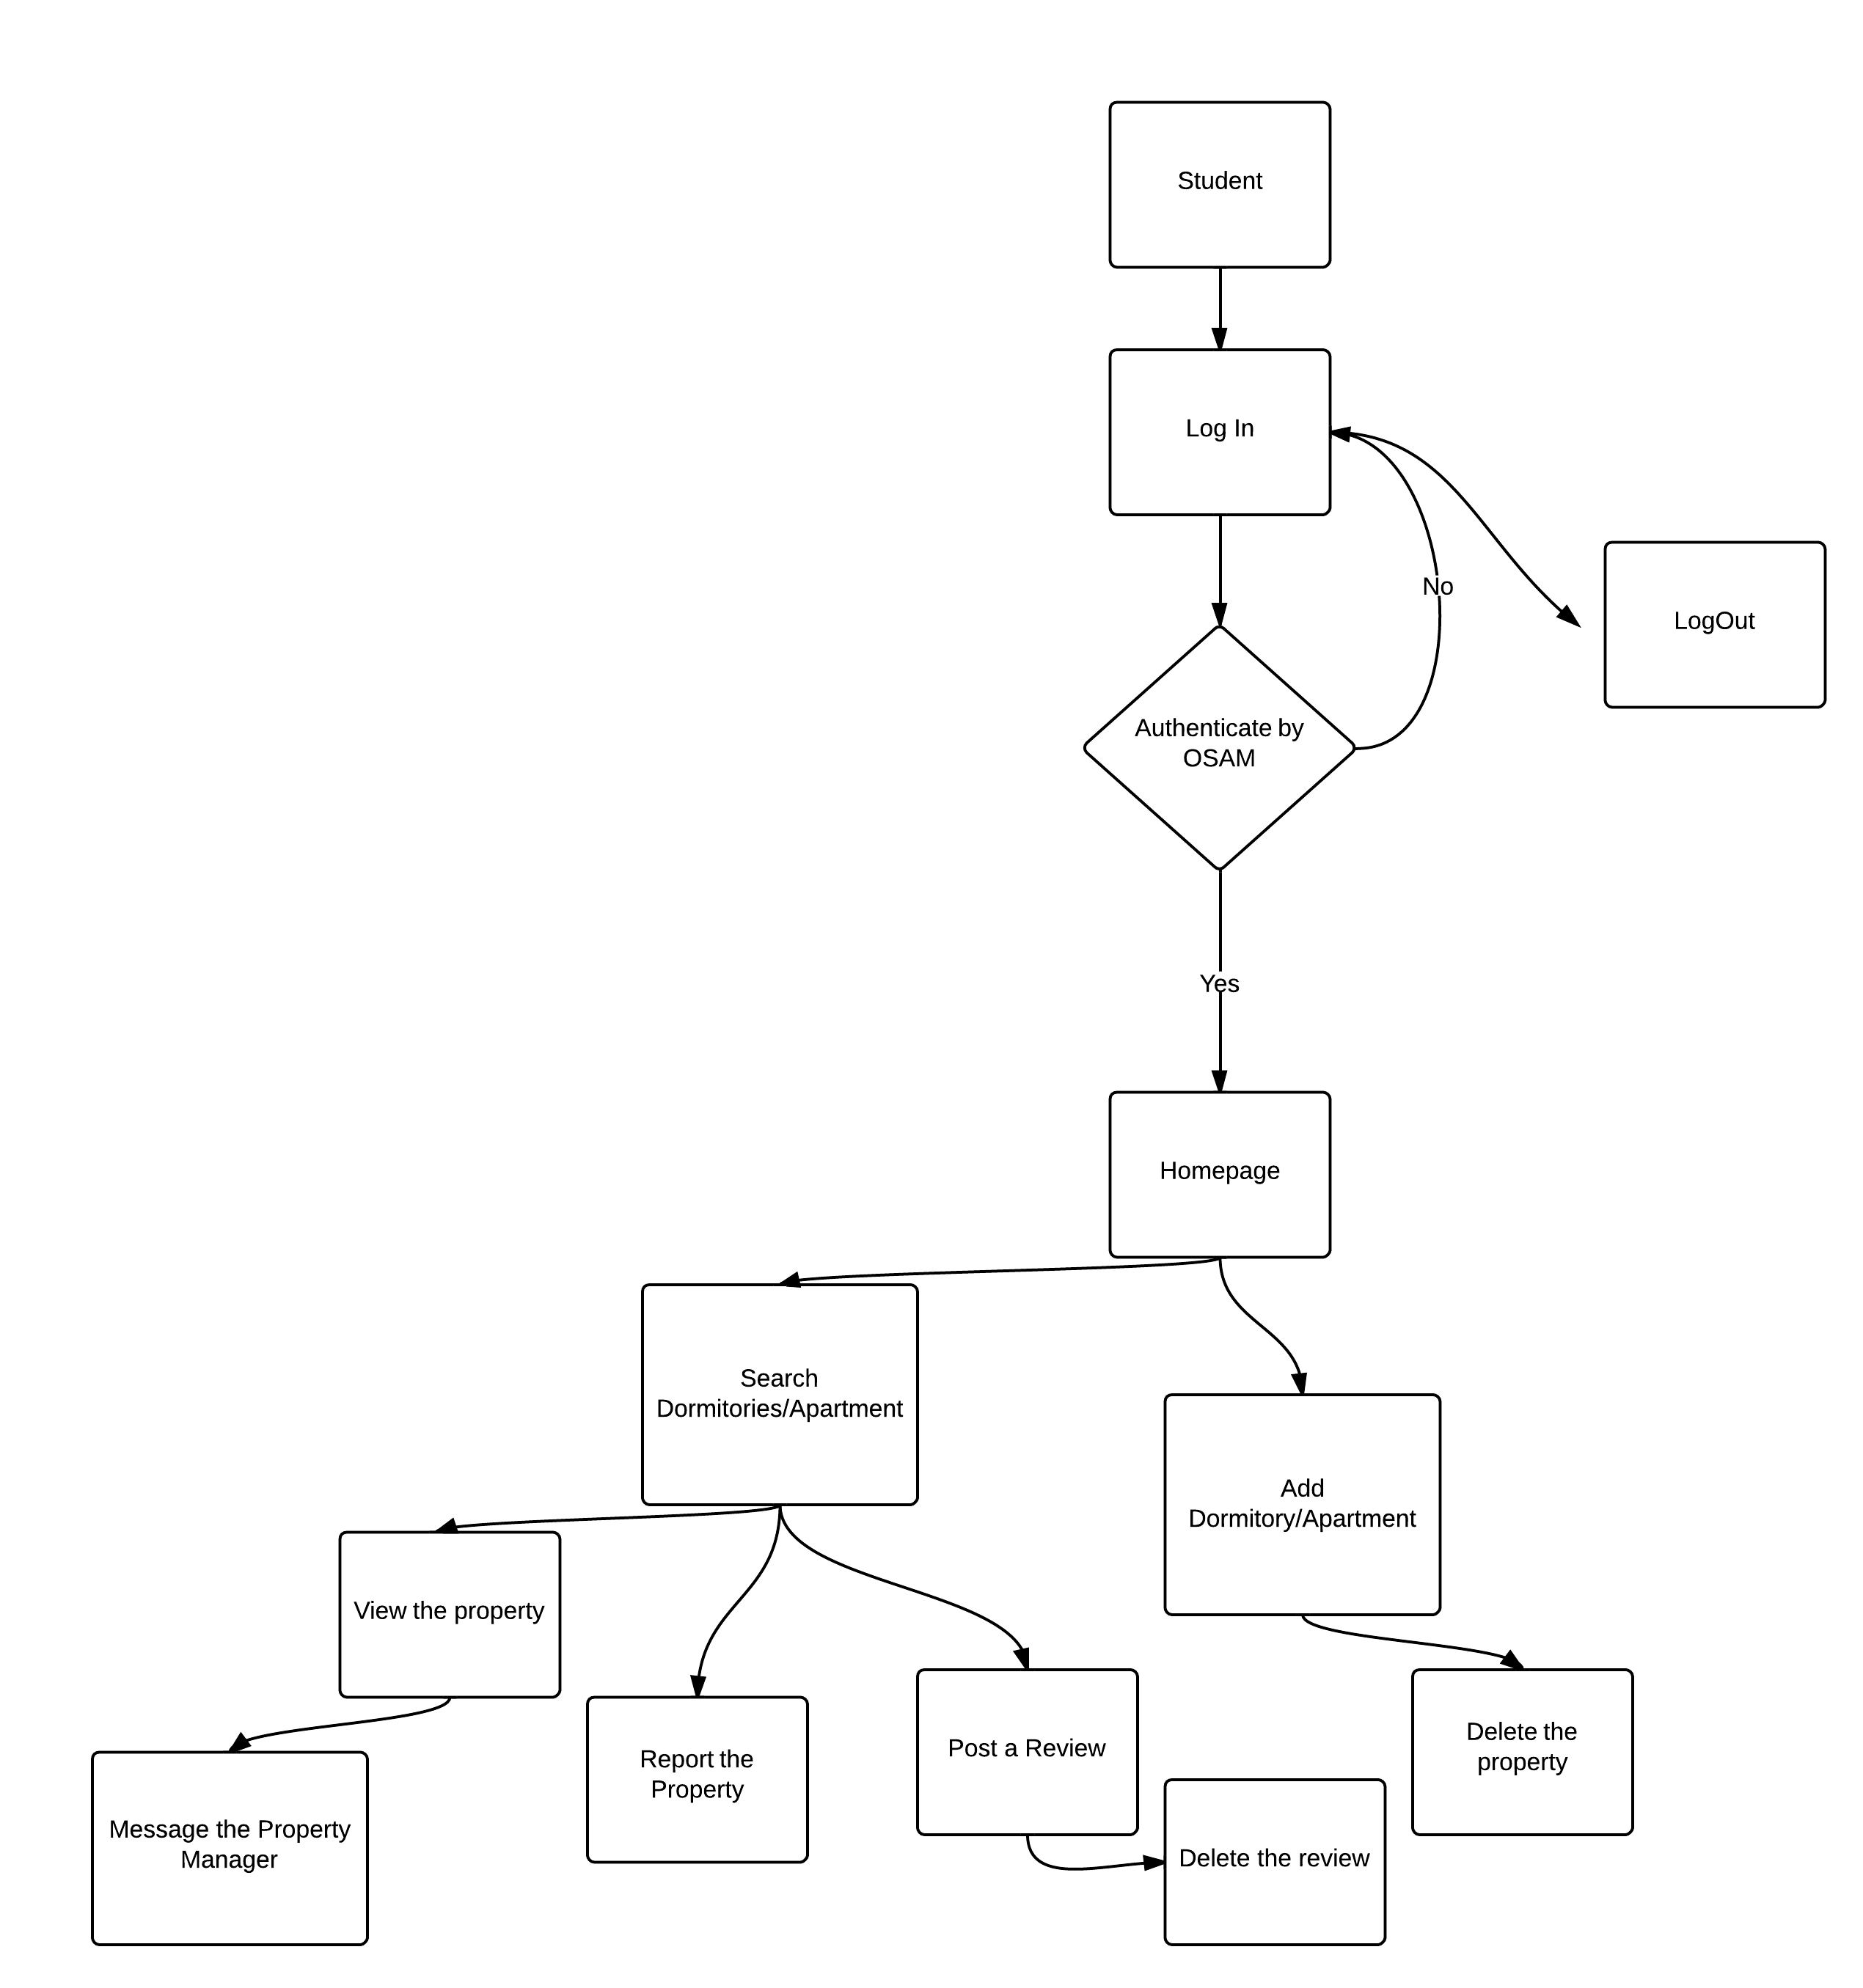
\includegraphics[width=9cm,height=12cm]{images/student.png}
			\caption{Student Workflow Diagram}
		
		\end{figure}
		\item A student is allowed to do the following functions:
			\begin{itemize}
				\item Add dormitories and apartments.
				\item Edit details about dormitory/apartment he/she added.
				\item Add and edit a review about the dormitories and apartments.
				\item Rate a dormitory and apartment
				\item Send a message to the property manager.
				\item Delete a dormitory and apartment he/she added.
				\item Report a dormitory and apartment.
				\item Search dormitories and apartments by :
					\begin{itemize}
						\item curfew
						\item users of the comfort rooms (shared / exclusive)
						\item bathing type (shower / pail)
						\item toilet facility (pail system, flush toilet, pit toilet) 
						\item deposit/advanced rent required
						\item rent payment (bank, cash, post-dated checks)
						\item sex (male only / female only / coed)
						\item distance of nearest sari-sari store in meters
						\item security features (has 24/7 guard, has night guard, has CCTV, landlord/landlady lives nearby, relies on good luck)
						\item electric/water billing (paid to landlord/landlady, paid to meralco/laguna water)
						\item internet availability (free wifi, paid wifi, bring your own, not allowed)
						\item transportation to university and approximate transportation time

					\end{itemize}
				\item View a dormitory and apartment.
			
		\item A property manager is allowed to do the following functions:
		\end{itemize}
			\begin{figure} 
			\centering
			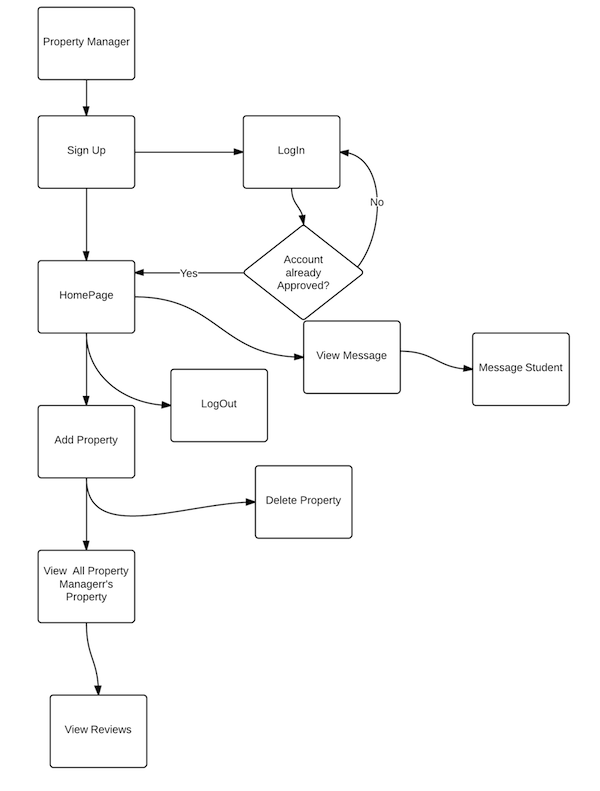
\includegraphics[width=10cm,height=12cm]{images/property.png}
			\caption{Property Manager Workflow Diagram}
			\end{figure}
			\begin{itemize}
				\item Add dormitories and apartments.
				\item Edit details about dormitory/apartment he/she added.
				\item Delete a dormitory and apartment he/she added.
				\item Search dormitories and apartments by :
					\begin{itemize}
						\item curfew
						\item users of the comfort rooms (shared / exclusive)
						\item bathing type (shower / pail)
						\item toilet facility (pail system, flush toilet, pit toilet) 
						\item deposit/advanced rent required
						\item rent payment (bank, cash, post-dated checks)
						\item sex (male only / female only / coed)
						\item distance of nearest sari-sari store in meters
						\item security features (has 24/7 guard, has night guard, has CCTV, landlord/landlady lives nearby, relies on good luck)
						\item electric/water billing (paid to landlord/landlady, paid to meralco/laguna water)
						\item internet availability (free wifi, paid wifi, bring your own, not allowed)
						\item transportation to university and approximate transportation time

					\end{itemize}
				\item View a dormitory and apartment.
			\end{itemize}
		\end{enumerate}
	\subsection{System Design}
		This phase involved the creation of Unified Modeling Language Diagram for the database system. Shown in Figure 4 is the Unified Modeling Language Class Diagram of the system.
		\begin{figure*}  
			
			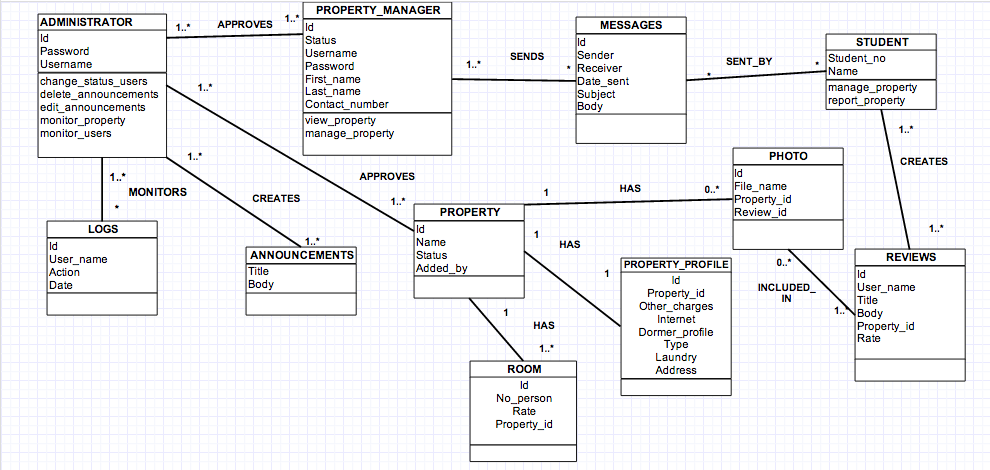
\includegraphics[width=20cm,height=9cm]{images/uml.png}
			\caption{Unified Modeling Language Class Diagram}
			\label{fig:erd}
	\end{figure*}

		The entity Administrator approves the existence of the entity Property Manager and Property. An Administrator is needed to create Announcements. When a Property Manager is approved by the Administrator, this entity can be able to add a Property and communicate with the students by sending messages.

		The entity Property has a Property Profile which includes all the details concerning the property. The Property also has rooms and photos. A property can have Reviews created by the Students. A student can include a photo in the review. A student can also add property.
	

\bibliographystyle{./IEEE/IEEEtran}
\bibliography{./cs190-ieee}
\nocite{*}



\end{document}
 
